% 共角共边 引入：△ABC，D∈AB, E∈AC，AD/AC=AE/AB（交叉），证 △ADE~△ACB
\documentclass[tikz,border=4pt]{standalone}
\usepackage{ctex}
\usepackage{amsmath}
\usetikzlibrary{calc}
\begin{document}
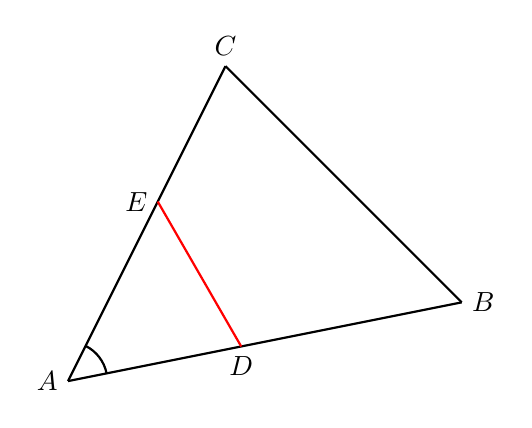
\begin{tikzpicture}[scale=1.0, thick]
  \coordinate (A) at (0,0);
  \coordinate (B) at (5,1);  % AB 长 ~5.1
  \coordinate (C) at (2,4);  % AC 长 ~4.47
  % 交叉对应：AD/AC = AE/AB. 取比例 k=0.5: AD=0.5*AC≈2.24, AE=0.5*AB≈2.55
  % D 在 AB 上, AD=2.24 -> D = A + (2.24/5.1)*(B-A)
  \coordinate (D) at ($(A)!0.44!(B)$);
  \coordinate (E) at ($(A)!0.57!(C)$);
  \draw (A)--(B);
  \draw (A)--(C);
  \draw (B)--(C);
  \draw[red] (D)--(E);
  \node[left] at (A) {$A$};
  \node[right] at (B) {$B$};
  \node[above] at (C) {$C$};
  \node[below] at (D) {$D$};
  \node[left] at (E) {$E$};
  % 公共角弧
  \draw ($(A)+(11.31:0.5)$) arc[start angle=11.31, end angle=63.43, radius=0.5];
\end{tikzpicture}
\end{document}
